\documentclass[10pt,a4paper]{article}
\usepackage[latin1]{inputenc}
\usepackage[margin=1in]{geometry}
\usepackage{amsmath}
\usepackage{amsfonts}
\usepackage{amssymb}
\usepackage{graphicx}
\usepackage{hyperref}

\usepackage{tikz}
\usepackage{algpseudocode}
\usepackage{forloop}
\newcounter{population}
\newcounter{numcol}

\usepackage{fancyhdr} % Headers and footers
\pagestyle{fancy} % All pages have headers and footers
\fancyhead{} % Blank out the default header
\fancyfoot{} % Blank out the default footer
\fancyhead[C]{Montana State University \quad $\bullet$ \quad CSCI 466 Artificial Intelligence \quad $\bullet$ \quad Group 21} % Custom header text
\fancyfoot[RO,LE]{\thepage} % Custom footer text

%----------------------------------------------------------------------------------------
%	TITLE SECTION
%----------------------------------------------------------------------------------------

\title{\vspace{-15mm}\fontsize{24pt}{10pt}\selectfont\textbf{CSCI 446 Artificial \\ [2mm]Intelligence Example Runs} \\} % Article title
\date{\today}
\author{
	\large
	\textsc{Roy Smart} \and \textsc{Nevin Leh} \and \textsc{Brian Marsh}\\[2mm] % Your name
}


%----------------------------------------------------------------------------------------


	
	
\begin{document}
	
	\maketitle % Insert title
	\thispagestyle{fancy}
	The five algorithms were run on an N=8 graph. Coloring at each step were recorded and displayed below. Please see the video files in the \texttt{videos} folder in this directory or at \href{https://www.youtube.com/playlist?list=PLiXOmiaruL8ih2YWsmPLjXUrztIMaAfSO}{\texttt{youtube.com}}
\section{Min Conflicts}


\begin{tabular}{c c c c }
	
	\includegraphics[scale=.10]{../results/min_conflicts/map_build/minconf_I00001.pdf}&
	\includegraphics[scale=.10]{../results/min_conflicts/map_build/minconf_I00002.pdf}&
	\includegraphics[scale=.10]{../results/min_conflicts/map_build/minconf_I00003.pdf}&
	\includegraphics[scale=.10]{../results/min_conflicts/map_build/minconf_I00004.pdf}\\
	
	\includegraphics[scale=.10]{../results/min_conflicts/map_build/minconf_I00005.pdf}&
	\includegraphics[scale=.10]{../results/min_conflicts/map_build/minconf_I00006.pdf}&
	\includegraphics[scale=.10]{../results/min_conflicts/map_build/minconf_I00007.pdf}&
	\includegraphics[scale=.10]{../results/min_conflicts/map_build/minconf_I00008.pdf}\\
	
	\includegraphics[scale=.10]{../results/min_conflicts/map_build/minconf_I00009.pdf}&
	\includegraphics[scale=.10]{../results/min_conflicts/map_build/minconf_I00010.pdf}\\


\end{tabular}	
	
\section{Simple Backtracking}
\begin{tabular}{c c c c }
	\includegraphics[scale=.10]{../results/backtracking_simple/map_build/bt_simple_I00001.pdf}&
	\includegraphics[scale=.10]{../results/backtracking_simple/map_build/bt_simple_I00002.pdf}&
	\includegraphics[scale=.10]{../results/backtracking_simple/map_build/bt_simple_I00003.pdf}&
	\includegraphics[scale=.10]{../results/backtracking_simple/map_build/bt_simple_I00004.pdf}\\
	
	\includegraphics[scale=.10]{../results/backtracking_simple/map_build/bt_simple_I00005.pdf}&
	\includegraphics[scale=.10]{../results/backtracking_simple/map_build/bt_simple_I00006.pdf}&
	\includegraphics[scale=.10]{../results/backtracking_simple/map_build/bt_simple_I00007.pdf}&
	\includegraphics[scale=.10]{../results/backtracking_simple/map_build/bt_simple_I00008.pdf}\\
	
	\includegraphics[scale=.10]{../results/backtracking_simple/map_build/bt_simple_I00009.pdf}&
	\includegraphics[scale=.10]{../results/backtracking_simple/map_build/bt_simple_I00010.pdf}&
	\includegraphics[scale=.10]{../results/backtracking_simple/map_build/bt_simple_I00011.pdf}&
	\includegraphics[scale=.10]{../results/backtracking_simple/map_build/bt_simple_I00012.pdf}\\
	
	\includegraphics[scale=.10]{../results/backtracking_simple/map_build/bt_simple_I00013.pdf}&
	\includegraphics[scale=.10]{../results/backtracking_simple/map_build/bt_simple_I00014.pdf}&
	\includegraphics[scale=.10]{../results/backtracking_simple/map_build/bt_simple_I00015.pdf}&
	\includegraphics[scale=.10]{../results/backtracking_simple/map_build/bt_simple_I00016.pdf}\\
	
	\includegraphics[scale=.10]{../results/backtracking_simple/map_build/bt_simple_I00017.pdf}&
	\includegraphics[scale=.10]{../results/backtracking_simple/map_build/bt_simple_I00018.pdf}&
	\includegraphics[scale=.10]{../results/backtracking_simple/map_build/bt_simple_I00019.pdf}&
	\includegraphics[scale=.10]{../results/backtracking_simple/map_build/bt_simple_I00020.pdf}\\
	
	
\end{tabular}


\section{Backtracking with Forward Checking}
Please note that the intermediate colorings represent an additive mixing of the 4 pure colorings.\\
\begin{tabular}{c c c c }
	\includegraphics[scale=.10]{../results/backtracking_forward/map_build/bt_forward_I00001.pdf}&
	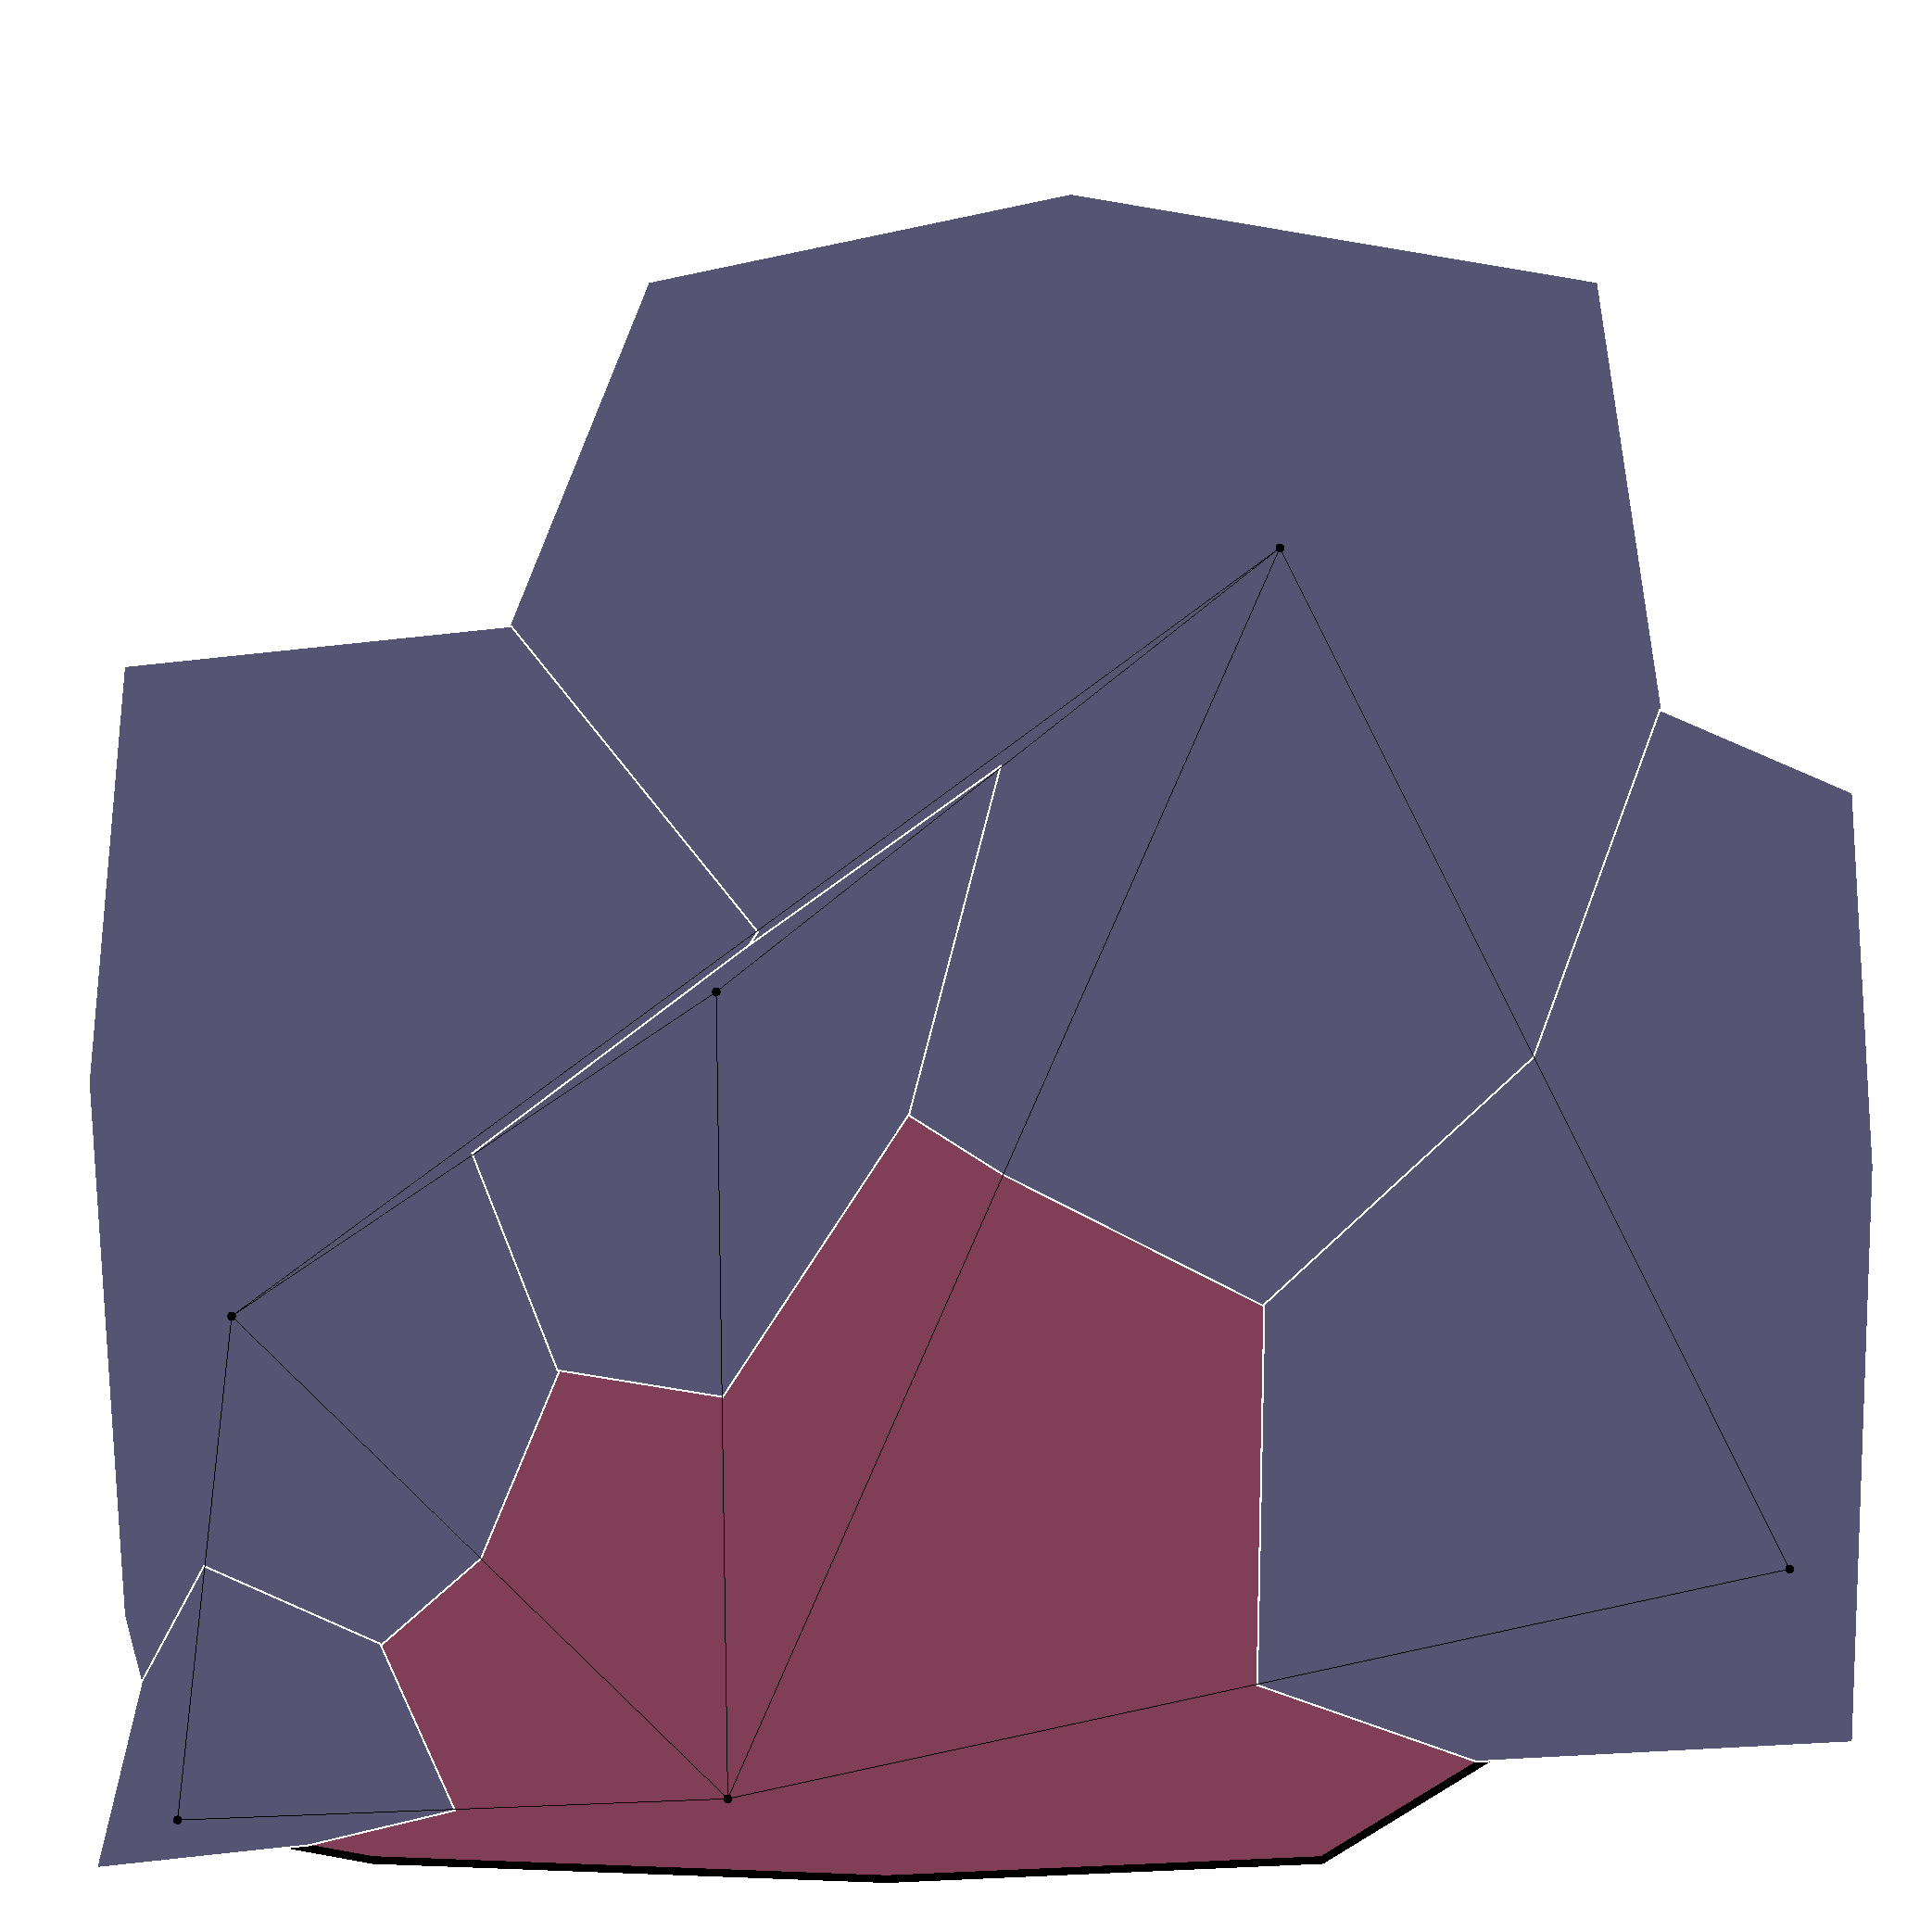
\includegraphics[scale=.10]{../results/backtracking_forward/map_build/bt_forward_I00002.pdf}&
	\includegraphics[scale=.10]{../results/backtracking_forward/map_build/bt_forward_I00003.pdf}&
	\includegraphics[scale=.10]{../results/backtracking_forward/map_build/bt_forward_I00004.pdf}\\
	
	
	\includegraphics[scale=.10]{../results/backtracking_forward/map_build/bt_forward_I00005.pdf}&
	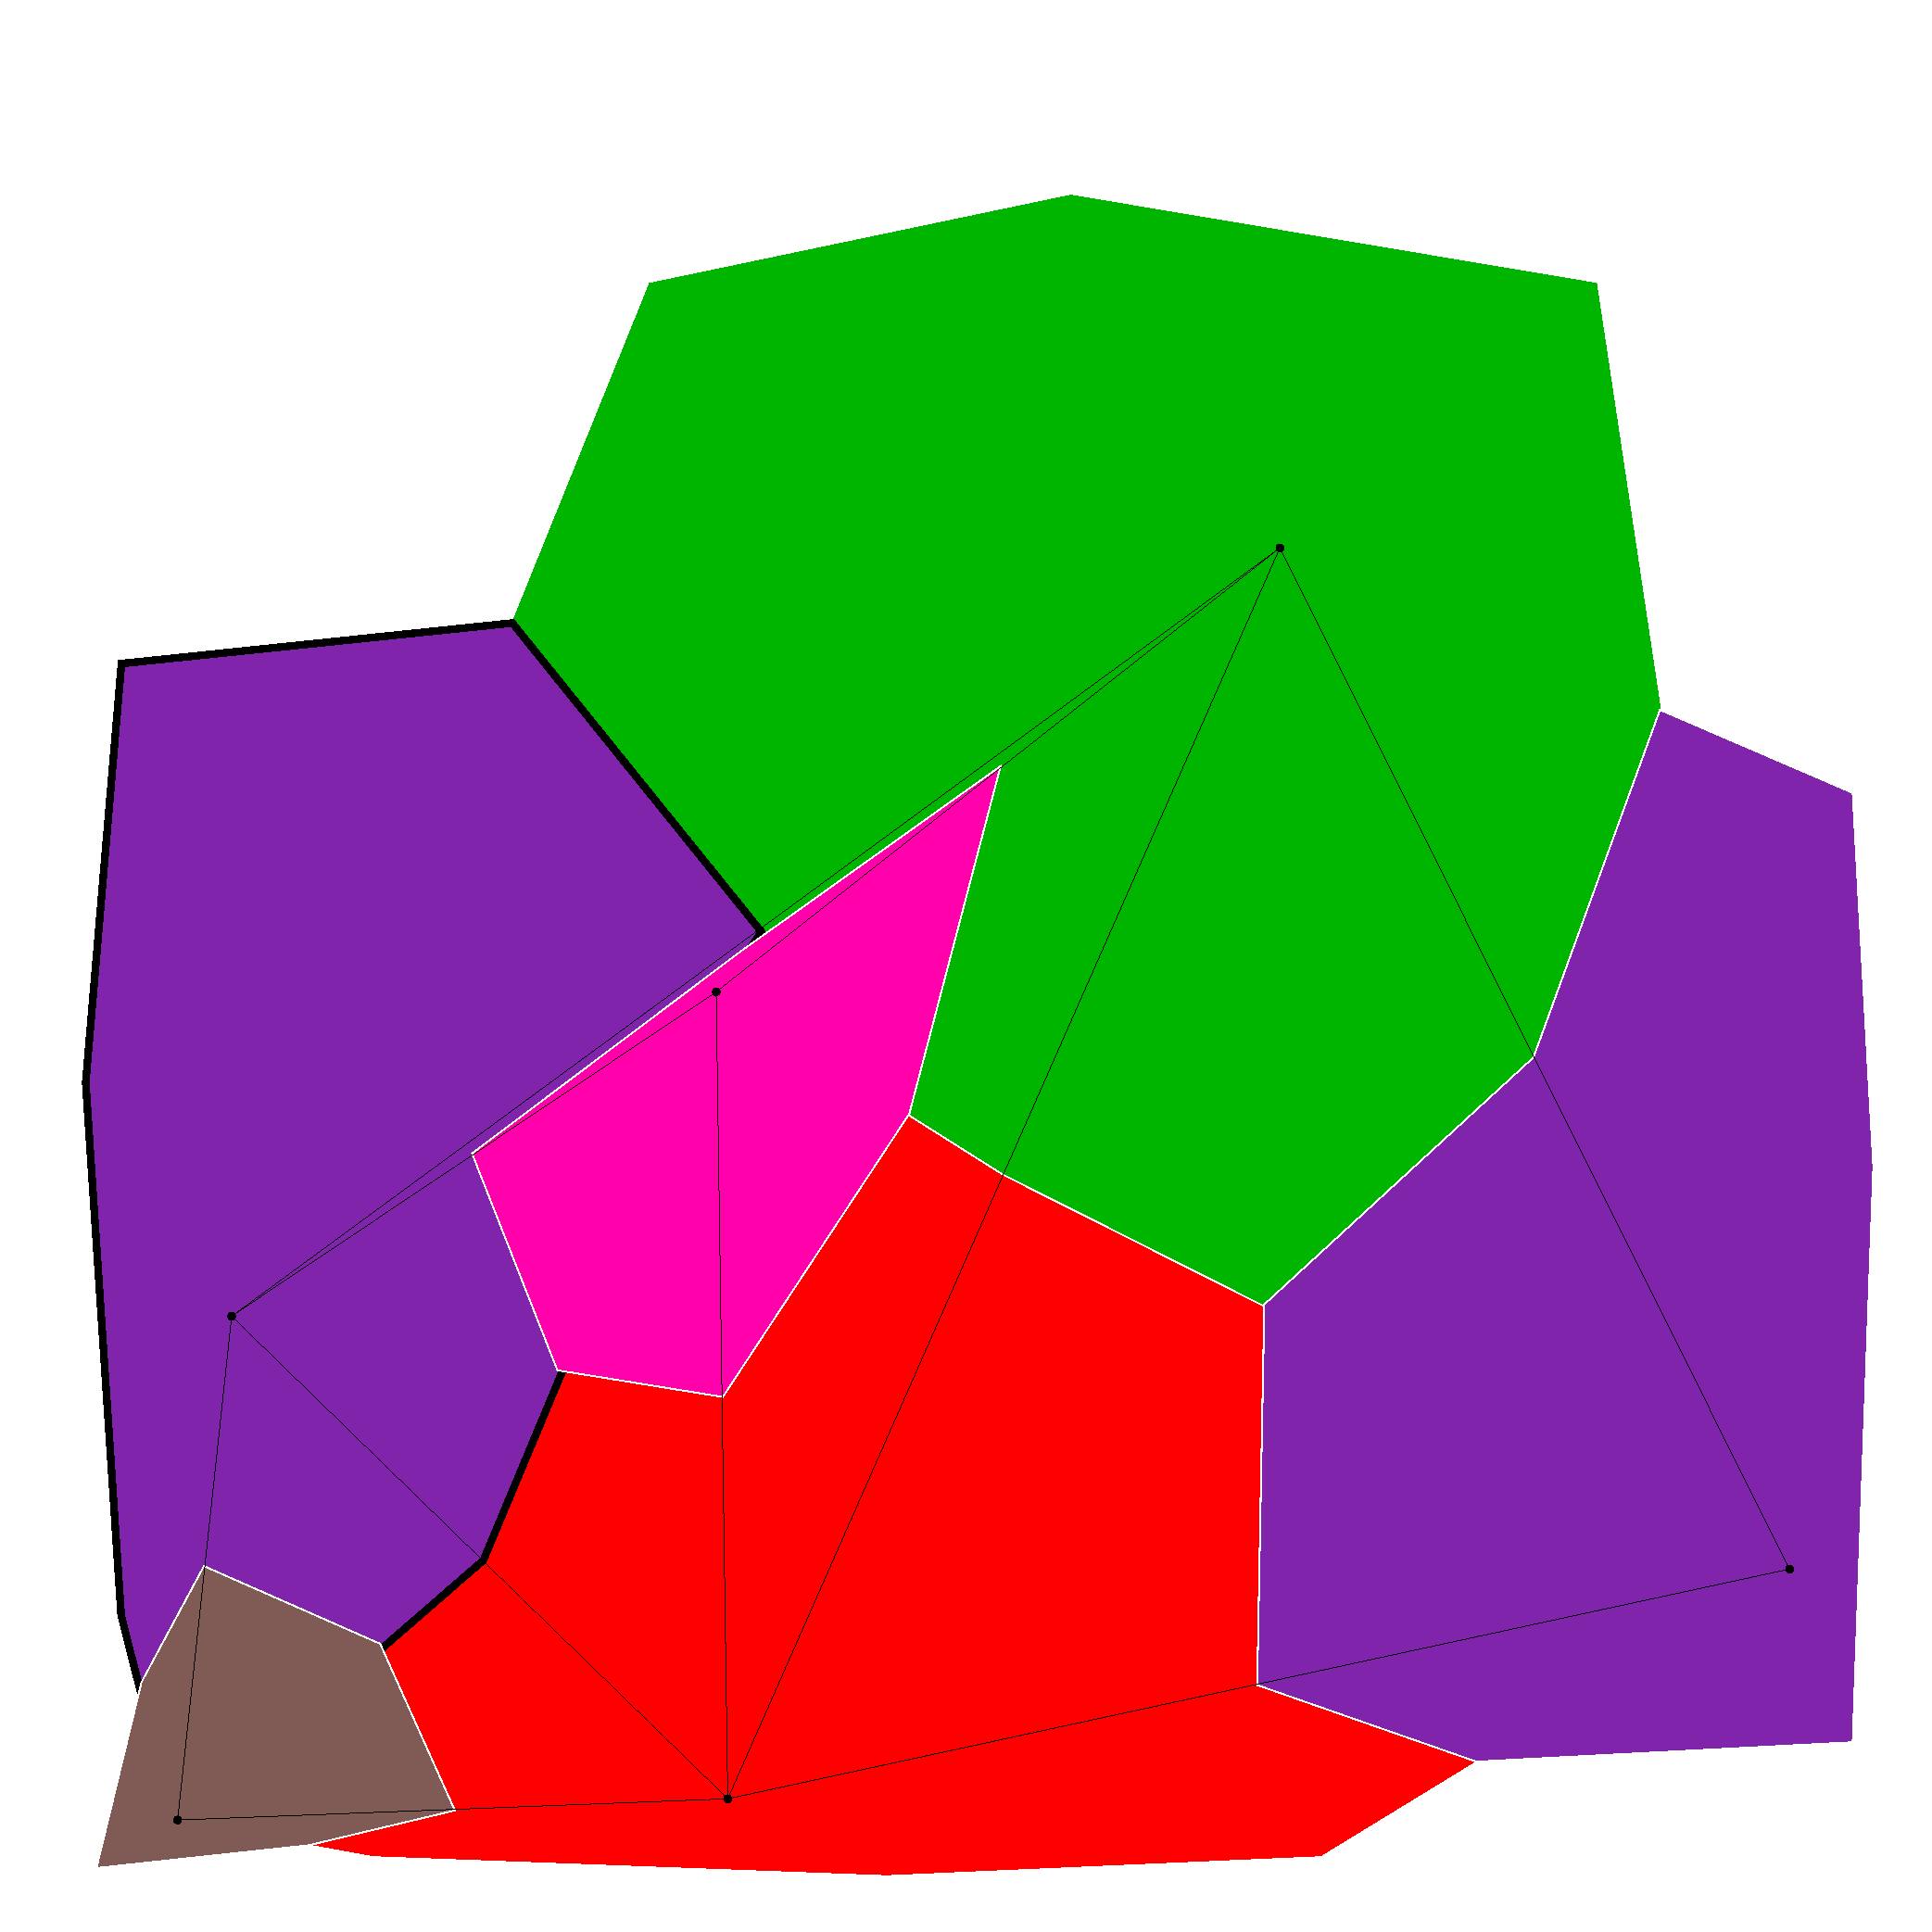
\includegraphics[scale=.10]{../results/backtracking_forward/map_build/bt_forward_I00006.pdf}&
	\includegraphics[scale=.10]{../results/backtracking_forward/map_build/bt_forward_I00007.pdf}&
	\includegraphics[scale=.10]{../results/backtracking_forward/map_build/bt_forward_I00008.pdf}\\
	
	\includegraphics[scale=.10]{../results/backtracking_forward/map_build/bt_forward_I00009.pdf}&
	\includegraphics[scale=.10]{../results/backtracking_forward/map_build/bt_forward_I00010.pdf}&
	\includegraphics[scale=.10]{../results/backtracking_forward/map_build/bt_forward_I00011.pdf}&
	\includegraphics[scale=.10]{../results/backtracking_forward/map_build/bt_forward_I00012.pdf}\\
	
	\includegraphics[scale=.10]{../results/backtracking_forward/map_build/bt_forward_I00013.pdf}\\
\end{tabular}


\section{Backtracking with Constraint Propagation}
Please note that the intermediate colorings represent an additive mixing of the 4 pure colorings.\\
\begin{tabular}{c c c c }
	\includegraphics[scale=.10]{../results/backtracking_mac/map_build/bt_mac_I00001.pdf}&
	\includegraphics[scale=.10]{../results/backtracking_mac/map_build/bt_mac_I00002.pdf}&
	\includegraphics[scale=.10]{../results/backtracking_mac/map_build/bt_mac_I00003.pdf}&
	\includegraphics[scale=.10]{../results/backtracking_mac/map_build/bt_mac_I00004.pdf}\\
	
	\includegraphics[scale=.10]{../results/backtracking_mac/map_build/bt_mac_I00005.pdf}&
	\includegraphics[scale=.10]{../results/backtracking_mac/map_build/bt_mac_I00006.pdf}&
	\includegraphics[scale=.10]{../results/backtracking_mac/map_build/bt_mac_I00007.pdf}&
	\includegraphics[scale=.10]{../results/backtracking_mac/map_build/bt_mac_I00008.pdf}\\
	
	\includegraphics[scale=.10]{../results/backtracking_mac/map_build/bt_mac_I00009.pdf}&
	\includegraphics[scale=.10]{../results/backtracking_mac/map_build/bt_mac_I00010.pdf}&
	\includegraphics[scale=.10]{../results/backtracking_mac/map_build/bt_mac_I00011.pdf}&
	\includegraphics[scale=.10]{../results/backtracking_mac/map_build/bt_mac_I00012.pdf}\\
	

\end{tabular}


\section{Genetic}
Please note that each picture shows the most fit individual from each generation. \\
\begin{tabular}{c c c c }
	\includegraphics[scale=.10]{../results/genetic/map_build/genetic_I00001.pdf}&
	\includegraphics[scale=.10]{../results/genetic/map_build/genetic_I00002.pdf}&
	\includegraphics[scale=.10]{../results/genetic/map_build/genetic_I00003.pdf}&
	\includegraphics[scale=.10]{../results/genetic/map_build/genetic_I00004.pdf}\\
	
	\includegraphics[scale=.10]{../results/genetic/map_build/genetic_I00005.pdf}&
	\includegraphics[scale=.10]{../results/genetic/map_build/genetic_I00006.pdf}\\
\end{tabular}

	
	
\end{document}